\documentclass[12pt,a4paper,twoside]{report}
\usepackage[pdfborder={0 0 0}]{hyperref}
\usepackage[margin=25mm]{geometry}
\usepackage{graphicx}
\usepackage{parskip}
\usepackage{enumerate}
\usepackage[utf8]{inputenc}
\usepackage{amsmath}
\usepackage{amsfonts}
\usepackage{float}
\graphicspath{ {Images/} }
\usepackage{subcaption}
\usepackage{algorithm}% http://ctan.org/pkg/algorithms
\usepackage{algpseudocode}% http://ctan.org/pkg/algorithmicx


% For temporarily splitting the document into multiple columns
\usepackage{multicol}

% Command for extracting the word count.
%\newcommand\wordcount{\input{word.count}}

\begin{document}

% Title Page
\begin{titlepage}
	\noindent
	\begin{minipage}[t][][t]{0.5\textwidth}
		
\includegraphics[width=40mm]{CamLogo.jpg}
	\end{minipage}
	\begin{minipage}{0.5\textwidth}
	\begin{flushright}
		\large
		\textit{Harry Graham}
		\\
		\textit{Christ's College}
		\\
		\texttt{hg402}
	\end{flushright}
	\end{minipage}
	
	\begin{center}
	\vspace{6cm}
	{\sc\large Computer Science Tripos - Part II Project\par}
	\vspace{0.5cm}
	{\huge\bf Deep Learning Techniques for Credit Card Fraud Detection\par}
	\vspace{0.5cm}
	{\large May 18, 2018 \par}
	\end{center}

\end{titlepage}

\pagestyle{plain}

% Proforma 
\section*{\huge Proforma}
\vspace{0.5cm}
{\large
\begin{tabular}{ll}
Name:               & \bf Harry Graham \\
College:            & \bf Christ's College \\
Project Title:      & \bf Deep Learning Techniques for Credit Card Fraud \\
			 & \bf Detection \\
Examination:        & \bf Computer Science Tripos -- Part II, June 2018 \\
Word Count:         &  \\
Project Originators: & H.~Graham \& B.~Dimanov \\
Supervisors:         & B.~Dimanov \& Dr M.~Jamnik
\end{tabular}
}

\section*{Original Aims of the Project}
The primary aim of the project was to implement and compare some deep learning techniques, alongside some baseline models, for credit card fraud detection (CCFD). More specifically, I aimed to experiment with two popular types of architecture, namely Convolutional Neural Networks (CNNs)  \cite{DBLP:journals/corr/SimonyanZ14a} and Generative Adversarial Networks (GANs). These have been successful in the image classification space and the aim of this project was to shed light on their use in the credit card fraud space. This kind of experimentation of predominantly image-based models, on single dimensional, time-series data is a relatively novel approach for CCFD.

\section*{Work Completed}
All of the core project aims set out in the proposal have been met, meaning results have been collated and evaluated across the three main components of the project: Baseline Models, CNN methods and GAN methods. 
I have also gone on to do some extension work relating to further investigation on the models I have experimented with. This is in the form of parameter tuning and further analysis not originally set out in the project proposal.

\section*{Special Difficulties}
None.


\newpage

% Declaration
\section*{Declaration}

I, Harry Graham of Christ's College, being a candidate for Part II of the Computer Science Tripos, hereby declare that this dissertation and the work described in it are my own work, unaided except as may be specified below, and that the dissertation does not contain material that has already been used to any substantial extent for a comparable purpose.

\vspace{1cm}
\begin{multicols}{2}

\rule{5cm}{0.15mm} \\
\leftline{\scshape{Signed}}

\columnbreak

\rule{5cm}{0.15mm} \\
\leftline{\scshape{Date}}

\end{multicols}


\tableofcontents

\pagestyle{headings} 

% Introduction
\chapter{Introduction}

Credit card fraud is a globally significant and increasing problem. According to the Nilson Report \cite{nilsonreport}, annual global fraud losses reached \$22.80 billion in 2016, up 4.4\% over 2015. Machine learning has contributed a lot to this problem over the years, helping to automatically learn to classify fraudulent transactions. However, this is still somewhat tedious and clearly, the money lost due to fraud is not decreasing. Not to mention, we still have this difficult business decision of when to draw the cutoff points between classifying fraud but perhaps allowing more benign transactions to be blocked.

A lot of machine learning concepts have been around for decades but ongoing research into deep learning architectures and their applications, makes for an interesting experimentation space. In this project I explore the performance of some particular models, focusing on deep learning, applied to the particular problem of credit card fraud detection (CCFD).

In particular, the aim is to shed light on the use of architectures that have had success in the image classification/generation space, in the context of non-image data i.e transactional vectors and time series data.
This is something that has recently seen some success \cite{wang2017time} and is novel to credit card fraud data. 
I first explore a set of baseline classifiers, which are primarily a handful of out-of-the-box supervised learning classifiers such as Random Forest. The point of these is to set the scene for experimenting with the data and to see what can be achieved with what is easily available, in other words without any 'deep' learning components. Here, I also establish techniques and methods for processing and evaluating the data i.e cross-validation, datapoint scaling, and data visualisation. 

Then the project shifts to experimenting with Convolutional Neural Networks (CNNs) \cite{DBLP:journals/corr/SimonyanZ14a} and Generative Adversarial Networks (GANs) \cite{2014arXiv1406.2661G}. The main aim of the project is to determine whether these can be applied to time-series data and in particular, the credit card fraud data. I experiment with two different variations of each, which I will outline in this dissertation. In the context of the GAN, I focus on whether this adversarial model is useful in learning the data before trying a semi-supervised, multitask learning approach in order to draw comparisons as a classification model.  

% Preparation
\chapter{Preparation} \label{preparation}

\section{Software Engineering}

This section details the project requirements and early design decisions that were made.

\subsection{Requirements}
The main success criteria of the project is outlined as follows:

\begin{enumerate}
   \item Baseline Models
   \begin{itemize}
     \item Compare a handful of supervised learning classifiers, from SciKit-Learn.
     \item Using metrics described in the Evaluation section of the project.
     \item Experiment with resampling techniques. 
     \item Implement appropriate cross-validation.
   \end{itemize}
   \item CNN Models
   \begin{itemize}
     \item Implement CNN version 1 - Single vector input approach.
     \item Implement CNN version 2 - Time series, sliding image window approach.
   \end{itemize}
   \item GAN Models
   \begin{itemize}
     \item Implement GAN version 1 - Dense generator network.
     \item Implement GAN version 2 - Using a CNN model from previous work as the generator network.
     \item Experiment with how GAN is used and how it performs on the data.
   \end{itemize}
\end{enumerate}

 These were all done more or less in order. Some work overlapped, namely work on auxiliary functionality to allow appropriate cross validation or data preparation etc. More details on specifics is outlined in the implementation chapter. 
  
\subsection{Tools and Technologies Used} \label{tools}

Below I describe and justify where necessary the tools and technologies that I used.

\subsubsection{Machine Learning}

I implemented work predominately making use of Keras\footnote{\href{https://keras.io}{https://keras.io}}(with TensorFlow\footnote{\href{https://www.tensorflow.org}{https://www.tensorflow.org}} backend) for CNN and GAN work and SciKit-Learn\footnote{\href{ http://scikit-learn.org/stable/}{ http://scikit-learn.org/stable/}} for baseline models and some general data manipulation/metric functions. 

The reasons for these choices were a mixture of good documentation, popularity \& ease-of-use. Using a TensorFlow backend meant that I could use GPU acceleration if needed. I used Keras as a TensorFlow wrapper, so I could avoid writing models completely from scratch but still giving me the flexibility to develop around models and customise to a large extent. Similarly with SciKit-Learn, which has a lot of helpful utility functions for evaluating models and processing data.

\subsubsection{Version Control and Project Tools}

I hosted my project in a repository on GitHub\footnote{\href{https://github.com/harrygraham/DeepLearning-CreditCardFraud}{https://github.com/harrygraham/DeepLearning-CreditCardFraud}}, used Git for version control, and used virtual environments with pip for project package management and requirements.

I made heavy use of Jupyter Notebooks for writing code in an experimental manner, with immediate execution and feedback. 


\subsubsection{Languages}

My project was entirely written in Python, using the libraries and APIs described previously. This is mainly due to the large ecosystem and documentation surrounding these machine learning libraries in python and also for the ease of use of tools such as Jupyter Notebooks for experimentation.

\subsection{Starting Point}

My project codebase was written from scratch, with the assistance of the tools and libraries mentioned above. Apart from a basic knowledge of supervised learning covered by the part IB Artificial Intelligence course, I had to learn about most of the models and best practises myself, through thorough reading around the topics. 


In terms of technologies, I had little prior experience with SKLearn and Keras/TensorFlow. I reviewed some documentation of these before-hand but I also took an agile approach to the project, whereby I consulted documentation as and when I needed, during my various milestone sprints. I had significant experience in Python, however, from a summer internship in industry as well as experience with Git.


\section{Convolutional Neural Networks}
Convolutional Neural Networks are a class of deep artificial neural networks, that have seen success in image recognition and other computer vision areas. Unlike typical neural networks, CNNs exploit spatial locality by shared weights. 

A CNN typically consists of an input layer, multiple hidden layers and an output layer. Hidden layers are usually convolutional layers, pooling layers and normalisation layers. 

\textbf{Convolutional Layer:}\\
A Convolutional Layer can take many parameters, the most prominent though are: 
\begin{enumerate}
  \item Input shape
  \item Kernel size
  \item Number of filters
  \item Stride size
\end{enumerate}

The \textbf{kernel size} defines the size of the filter that will be moved over the input shape, shifting by an amount defined by \textbf{stride size}. The \textbf{number of filters} simply defines how many separate filters we initialise and convolve with the input, to give multiple outputs. Convolving a filter with an input is essentially taking the dot product of all overlapping cells between the input and the filter, thus producing a single value in the output shape. 

This can be visualised with an example as follows:\\

\begin{figure}[H]

\centering
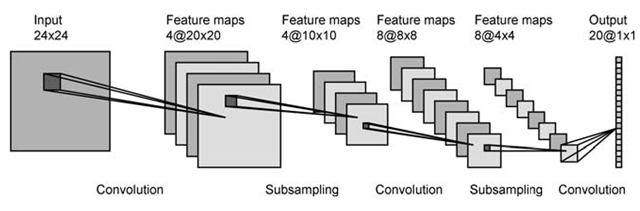
\includegraphics[width=\textwidth]{CNN-Example}
\caption{Example of a CNN network}
\end{figure}

We see here that in the first convolutional layer, the input shape is 24x24 and the kernel size is 5x5, which strides over the input shape to produce 4x(20x20) shapes. Here the number of filters was 4, which is why 4 outputs have been produced. Also, typically the stride size is 1. In this 24x24 input, with a 5x5 filter we can have $(24-5+1)$ possible positions of the filter in one direction. 

\textbf{Subsampling / Pooling:}\\
Subsampling is essentially taking the average across a group of cells to produce a smaller shape. This therefore produces the same number of 'feature maps' but smaller in size. 

\textbf{Fully Connected Layers:}\\
Fully Connected Layers (FCs) take all the feature maps from a convolutional layer and stack them all together in a traditional neural network in which every node is connected to every other node (fully connected). This then allows the network to learn the relationships between small parts of the image (or input in general) on a fine grained level. 


\section{Generative Adversarial Networks}
GAN is a framework proposed by Ian Goodfellow, Yoshua Bengio and others in 2014. The idea is that we have two networks: a generator and a discriminator. The generator network tries to produce,  from random noise,  data in the form of the training data we want. This could be an image, in the common use-case, or in this one, a fraudulent transaction vector. The discriminator, takes in real-life data (from the training set) and also the generated data from the generator network. The discriminator tries to determine whether the current input is real or generated. Effectively these two networks play a game with each other: the generator tries to fool the discriminator whilst the discriminator tries to catch out the generator. This continues until each network doesn't get any better and the GAN stabilises. Figure 2.1 represents an overview of a GAN network.

\begin{figure}[H]

\centering
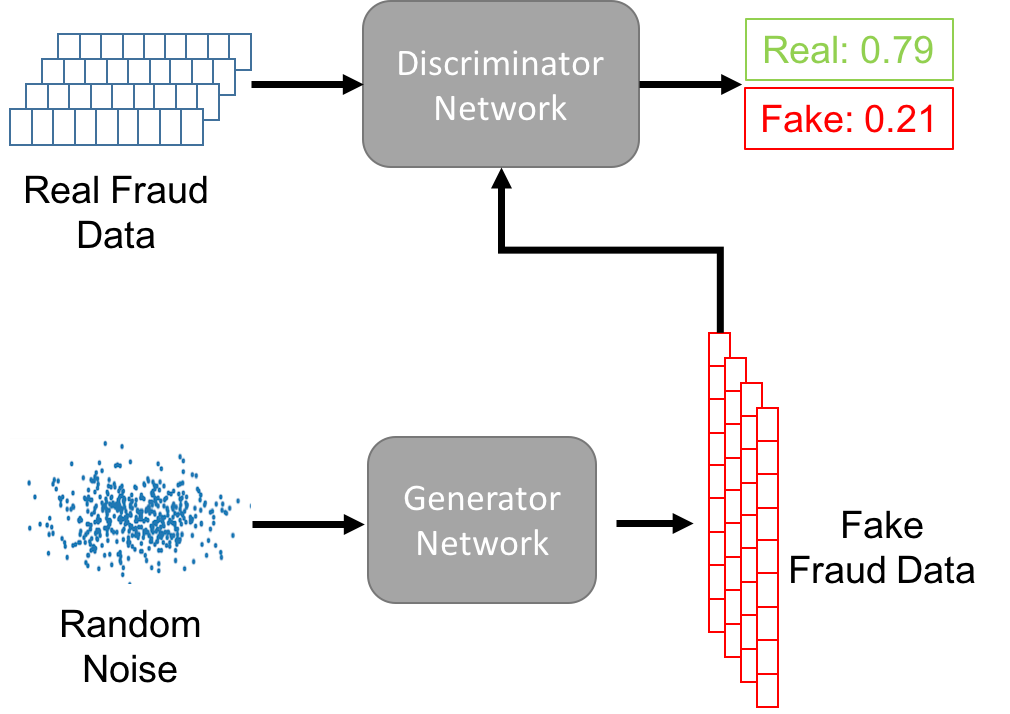
\includegraphics[width=\textwidth]{GAN-Overview}
\caption{Overview of a GAN network}
\end{figure}

Mathematically, we can define the following quantities:

$$X_{x\sim p_\text{data}(x)} = \text{Sample from distribution of real data} $$
$$Z_{z\sim p_\text{z}(x)} = \text{Sample from distribution of generated data} $$
$$G(z) = \text{Generator Network}$$
$$D(x) = \text{Discriminator Network}$$
The process of training for a GAN is like a min-max game between the two networks, and can thus be represented by the following value cost function:
$$\min _ { G } \max _ { D } V ( D ,G )$$
where 
$$V ( D ,G ) = \mathbb { E } _ { x \sim p _ { d a t a } ( x ) } [ \log D ( x ) ] + \mathbb { E } _ { z \sim p _ { z } ( z ) }[ \log ( 1- D ( G ( z ) ) ] $$
The first term in this equation represents the quantity of the real-distributed data passed through the discriminator network. The discriminator tries to maximise this such that $D(x)\rightarrow 1$. The second term represents generated data passed through the discriminator. The generator tries to minimise such that $D(G(z))\rightarrow 1$ (i.e the discriminator is fooled by the generated sample).

The steps for training a GAN can be outlined as followed:
\begin{enumerate}[Step 1:]
  \item 
  \begin{enumerate}
  \item Take a batch of real data and train discriminator to correctly predict them as real
  \item Take a batch of generated data and train discriminator to correctly predict them as fake
\end{enumerate}
  
  \item Freeze the training of the discriminator network
  \item Generate a batch of fake data and use the frozen discriminator to train the generator
  \item Repeat the above for n epochs until neither network makes any further improvments
\end{enumerate}

In summary, we alternate between training of the discriminator to correctly determine real or fake data and training the generator on fooling the discriminator. The reason for freezing the weights of the discriminator while we train the generator is exactly so that we don't alter the weights during this process and the generator can use the current state of the discriminator to become better.

\section{Machine Learning Evaluation Practices}
Here I describe some of the main machine learning evaluation concepts that I had to have a clear idea of, prior to implementation of this project. 

\subsection{Train and Test Splits}
Let's say we have \textbf{\textit{m}} examples $ \mathbf { x } _ { 1} ,\mathbf { x } _ { 2} ,\dots ,\mathbf { x } _ { m }$ each in $\mathbb { R } ^ { n }$. In a supervised learning problem, we also have \textbf{\textit{m}} labels $\left\{ y _ { 1} ,y _ { 2} ,\dots ,y _ { m } \right\}$ in a set \textbf{\textit{Y}}.\\
In machine learning we wish to find a hypothesis $h : \mathbb { R } ^ { n } \rightarrow Y$ that is defined by a vector of weights \textbf{\textit{w}}. It is then common to write $h _ { w } ( x )$.\\

We define a training set as $\mathbf{s} = [(\mathbf { x } _ { 1}, \mathbf { y } _ { 1}),(\mathbf { x } _ { 2}, \mathbf { y } _ { 2}),\dots,(\mathbf { x } _ { m}, \mathbf { y } _ { m})]$.
 
When training a model, to try and achieve our $h _ { w } ( x )$, we use data from the training set. When we train a model, it will often report some metrics or loss function to reflect how the performance increased during the training process. 

The problem with this however is that our model may not perform well on \textbf{unseen} data. In other words, it might not \textbf{generalise} well. To overcome this, it is good practise to preserve a testing portion of the data, called the test set, that is not used in the training process. The test set is then used to evaluate how the model performs after training. 

\begin{figure}[H]

\centering
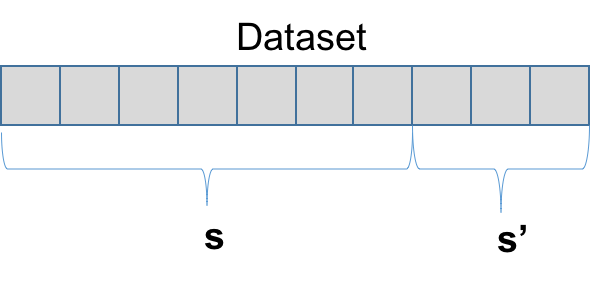
\includegraphics[scale=0.8]{train-test-split}
\caption{A 70:30 train test split of data.}
\end{figure}

\subsection{Cross-validation}

Cross-validation takes this a step further. The hypothesis of our model may in fact generalise and perform better on some portions of the data over others and thus performing just one split, may not give the most confident results. Also, when performing these train-test splits, the element of randomness in the split can work against us as even if we average this process say 3 times, it is likely that there is some overlap in the runs and we are not really using the data available to its full capacity. 

\begin{figure}[H]

\centering
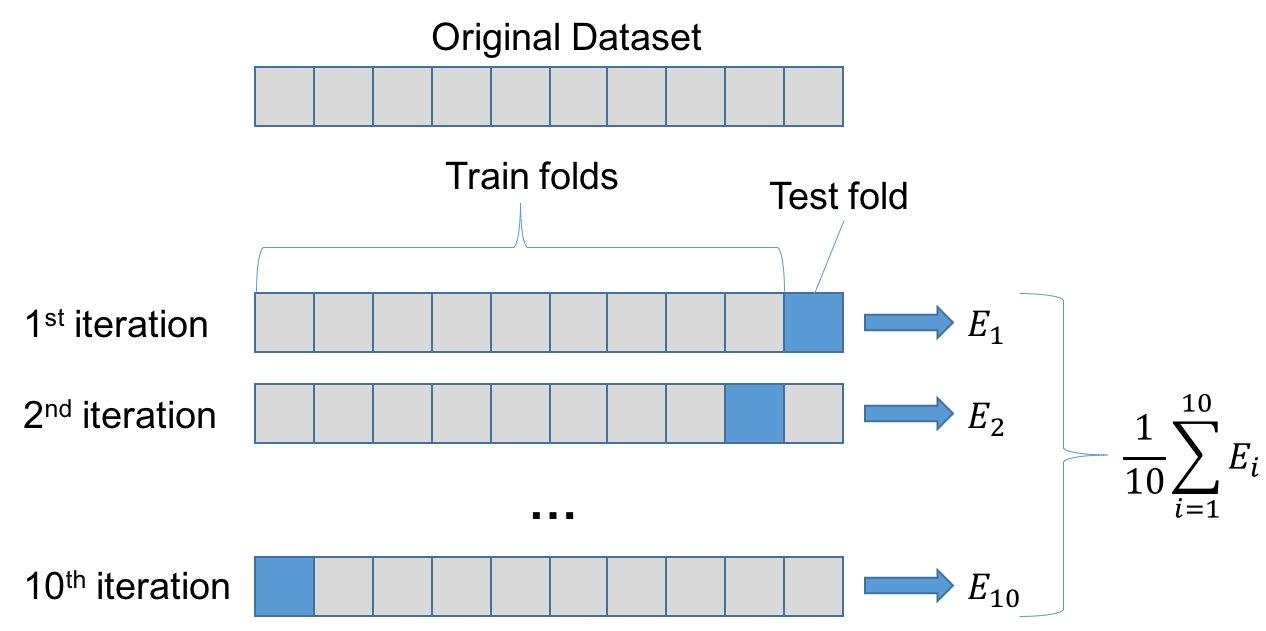
\includegraphics[scale=0.8]{cross-val}
\caption{K-Fold Cross Validation.}
\end{figure}

\subsection{Resampling Methods}

During the baseline work of the project I also experiment with resampling methods. These are ways of balancing the dataset such that the ratio of positive class to negative class is brought to 50:50. I do this to give an example of how these methods affect our results before moving onto the deep learning architectures. 
The three main methods I explored were:

\begin{enumerate}
  \item Undersampling 
  \item Duplicate Oversampling
  \item Synthetic Minority Oversampling Technique (SMOTE)
\end{enumerate}

\subsubsection{Undersampling}
Undersampling is the process of reducing the majority class down to a lower amount, to balance more with the minority class. This can be achieved by randomly removing samples until the ratio is 50:50 or another specified amount. 


\subsubsection{Duplicate Oversampling}
Duplicate Oversampling is a naive method of increasing the amount of the minority data class, to match that of the majority. This works by taking existing minority data points and simply duplicating them.

\subsubsection{SMOTE}
Synthetic Minority Oversampling Technique (SMOTE) is another method of increasing the amount of the minority data but not by duplication as before. SMOTE takes the $k$ nearest neighbours of a data point, randomly selects one of these k neighbours and creates a vector between the two. Then a new, synthetic data point is created some random distance along this vector line, by an amount in the range $[0,1]$.

\subsubsection{Cross-validating Correctly}
When employing oversampling techniques, this completely affects the way we handle cross-validation. It no longer is valid to simple oversample the dataset and then perform cross-validation. The reason for this is the potential of overfitting. Figure~\ref{fig:oversample-before} shows what can happen in this situation. 

\begin{figure}[H]
\centering
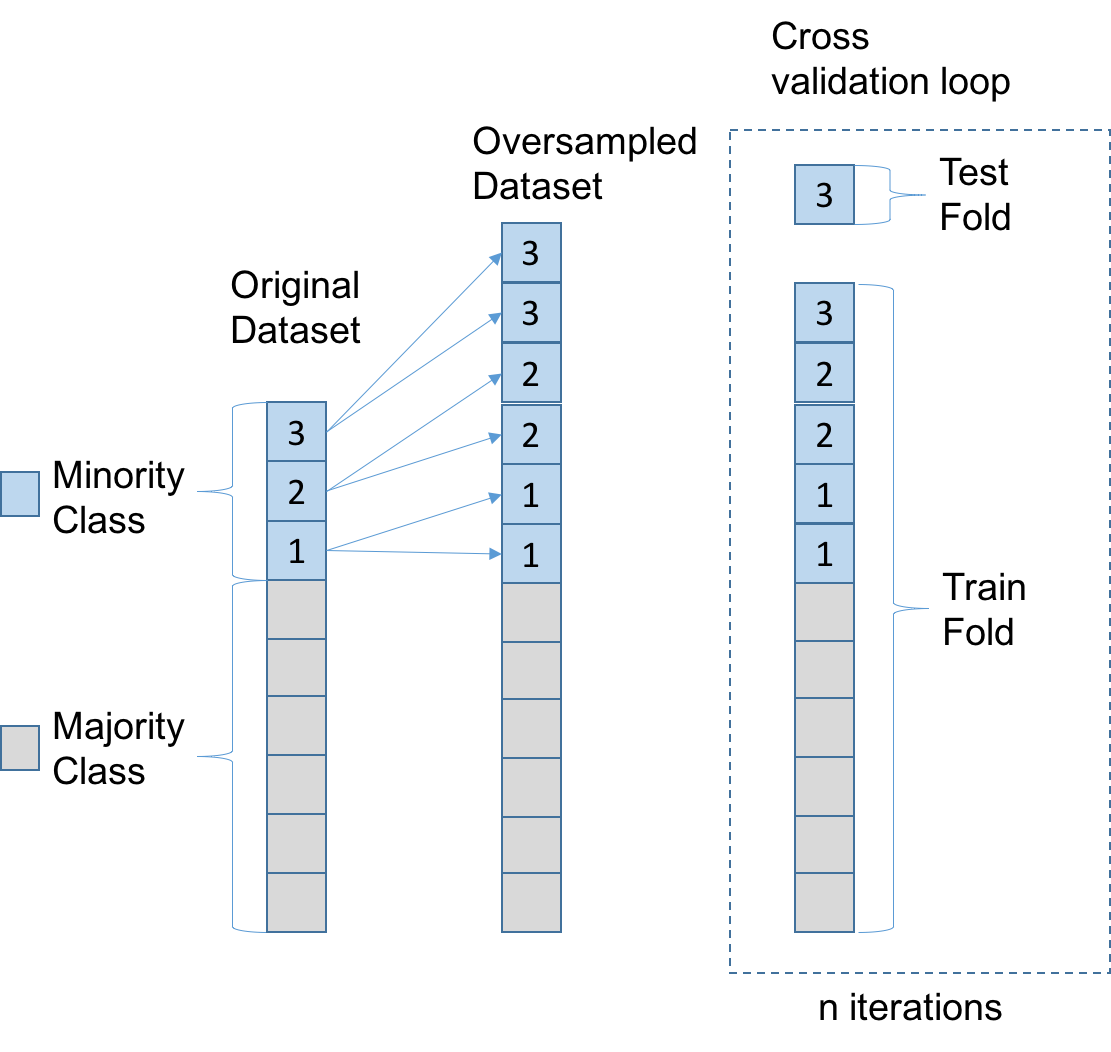
\includegraphics[scale=0.8]{oversample-before}
\caption{Oversampling OUTSIDE the cross-val loop.}
\label{fig:oversample-before}
\end{figure}

Inside the cross-validation loop, the current train-test folds split means that some of the oversampled minority class (node 3) that was portioned into the test set is also in the training set. This means that our model would have seen this data during the training process and will therefore have a bias during the testing and evaluation phase as it already knows how to classify this data. 

It is therefore crucial that this is adapted such that any oversampling occurs inside the cross-validation loop, and not before/outside it. Figure~\ref{fig:oversample-after-1} and Figure~\ref{fig:oversample-after-2} represent the correct way to handle this, for $n=1$ and $n=2$ respectively. For every iteration of the loop, we split the data into train-test first and then oversample the training data fold only. This preserves the testing fold, keeping a portion of the original dataset untouched, for evaluation. This is a lot more effective in testing the generalisability of a model.

\begin{figure}[H]
\centering
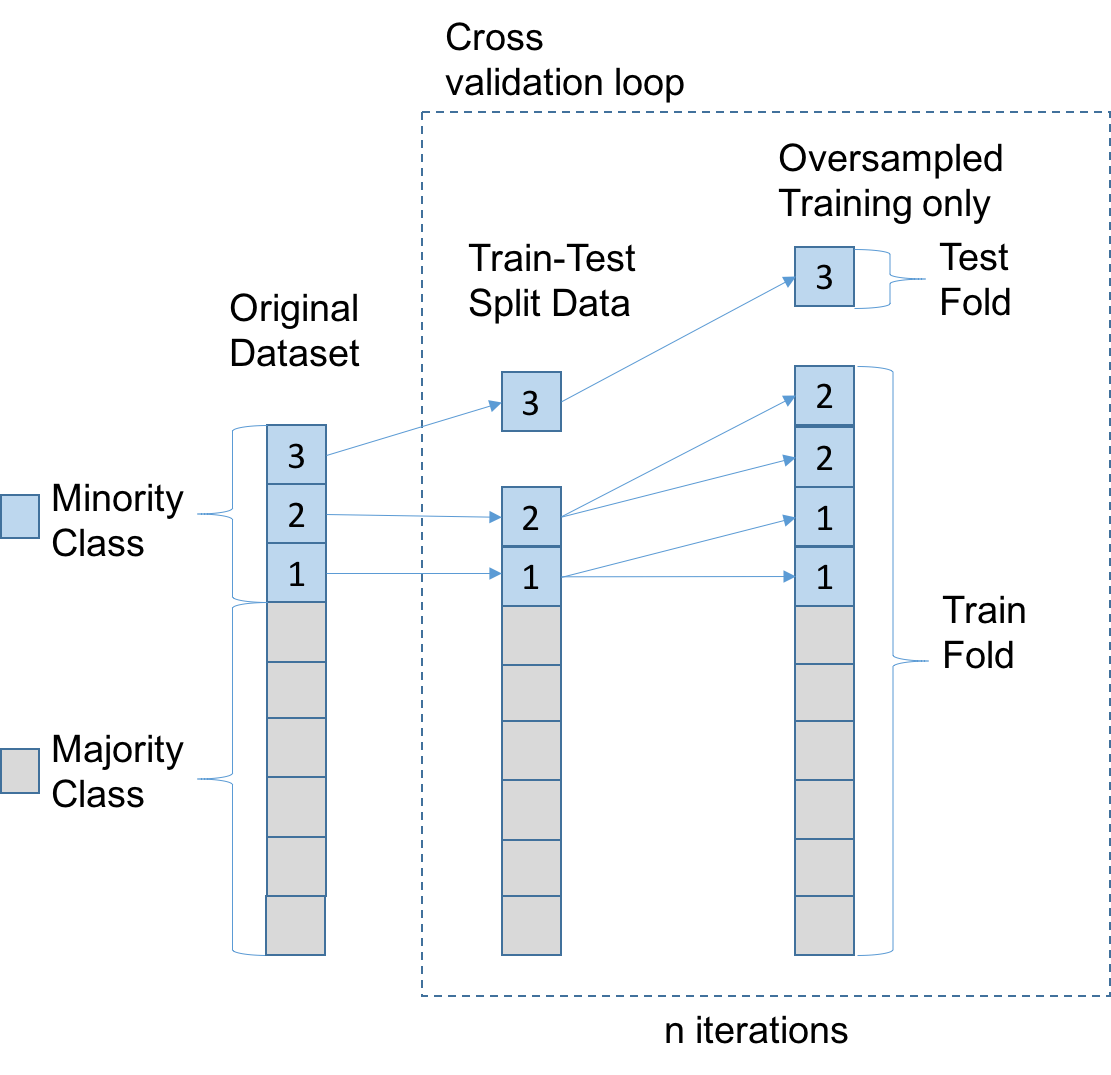
\includegraphics[scale=0.6]{oversample-after-1}
\caption{Oversampling INSIDE the cross-val loop [n=1].}
\label{fig:oversample-after-1}

\centering
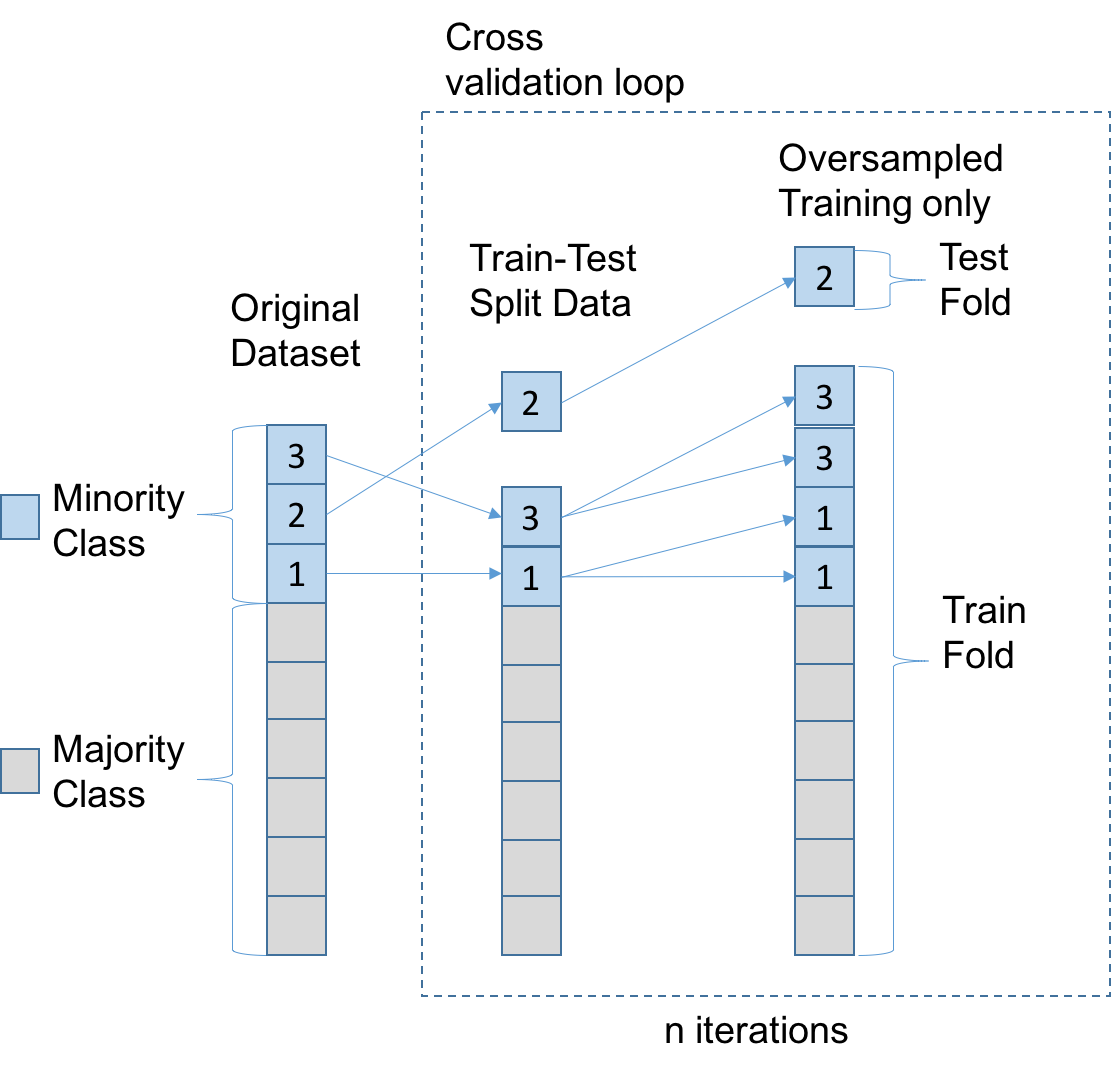
\includegraphics[scale=0.6]{oversample-after-2}
\caption{Oversampling INSIDE the cross-val loop [n=2].}
\label{fig:oversample-after-2}
\end{figure}

% Implementation
\chapter{Implementation}
\section{Models Overview}

\begin{figure}[H]
\centering
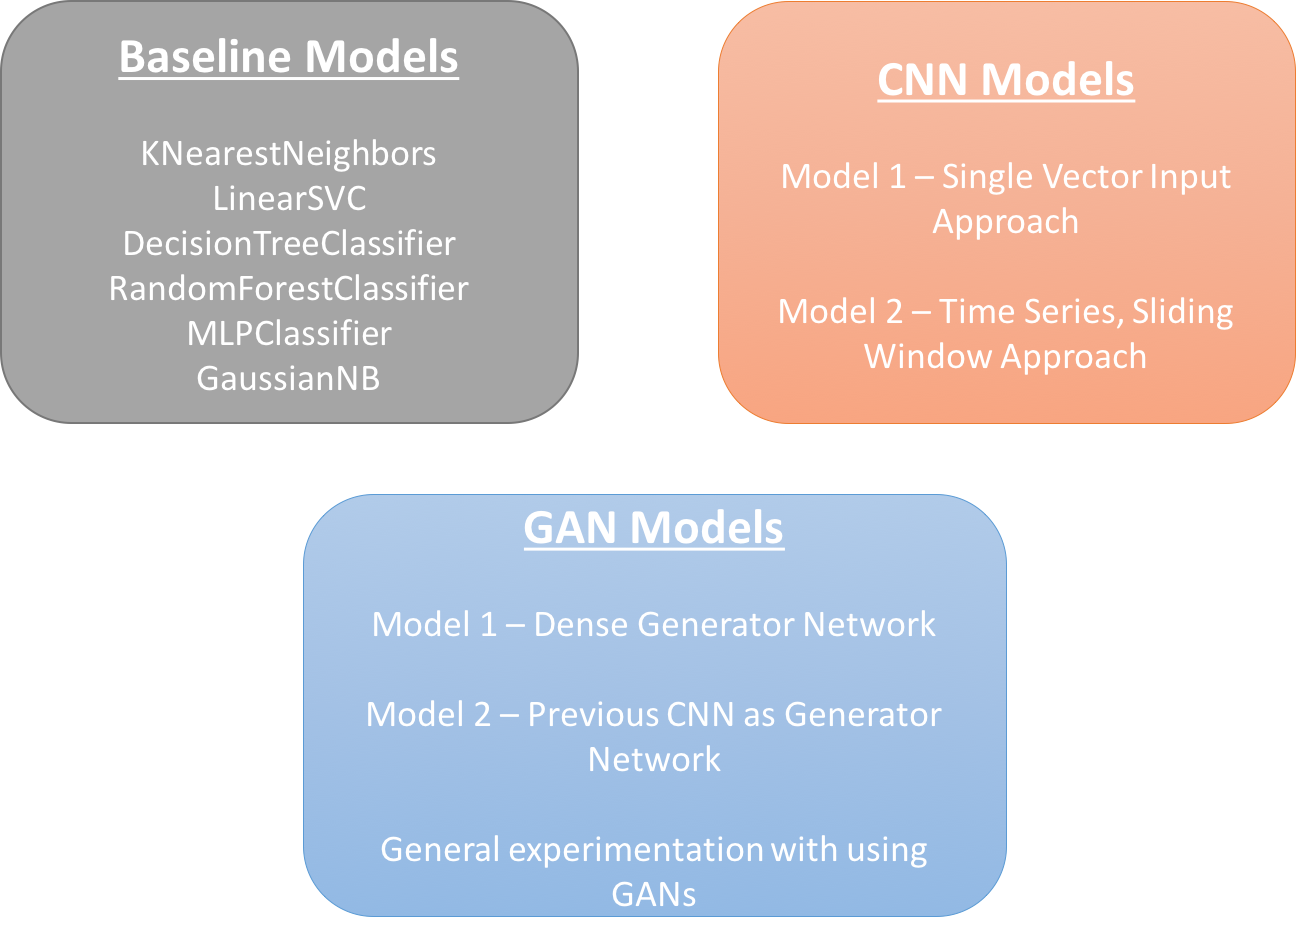
\includegraphics[scale=0.8]{models_overview}
\caption{Overview of models experimented with.}
\label{fig:models_overview}
\end{figure}

\section{Baseline Models}
\subsection{Data Preparation}

\textbf{Feature Scaling}\\

Standardisation involves rescaling the features such that they have the properties of a standard normal distribution with a mean of zero and a standard deviation of one. This is very important in machine learning when features can be a lot larger in magnitude than others. For example, if one feature is age and another is salary in USD then these two quantities will be on different ranges and the salary feature may negatively impact classifier algorithms by deeming that feature to be more important and confusing the weights assignment. Scaling solves this problem. 

Therefore one of the first steps was to scale the features, which I did using StandardScaler from SKLearn. 

\textbf{Feature Engineering}\\

In many machine learning and data science applications, feature engineering is something used to add additional features based on calculations and domain knowledge of the data. In this case, though, as the data is already post-PCA and the time-series span of the transactions is only over 2 days. I decided not to do any feature engineering and to just employ algorithms on the original dataset features.

\textbf{Sanity Checks}\\

Also, I checked the data to see if any values were missing, or null. This was to ensure that the data was clean to be passed through machine learning networks. There were no missing data in this case.

\subsection{Cross Validation Function}

Defining my own cross-validation function early on was a crucial step in this project. As explained briefly in the preparation chapter, the way in which cross-validation is performed is very important to ensure no overfitting occurs and that the results are as confident as they can be. As far as implementation is concerned, It was not enough to use the built in SKLearn cross-val function as it did not provide enough granularity in it's output. I wanted very specific metrics and not to mention, I needed to resample data in the correct place which meant I needed to define my own function, based on the standard library which uses Stratified KFold. This essentially means that the splitting of the data in each fold of the KFold procedure, contains at least some portion of the underrepresented class. This is important as it would be very common that some folds don't contain any of the minority class. 

The function uses a utility function from SKLearn, \textbf{precision\_recall\_f1}, which simply reports the precision, recall and f1-score for predicted values. You give it a set of predicted values and the set of true values and it calculates the metrics. I use this inside my function to report the metrics we are interested in, something I could not do originally. 

\begin{algorithm}[H]
\caption{Cross-Validation function }\label{cross-val}
\begin{algorithmic}[1]
\Procedure{custom-cross-val}{$X, Y, CLF, N$}

   \State $skfolds\gets \textbf{StratifiedKFold}(n\_splits = N)$\\
   
   \State $precisions\gets []$
   \State $recalls\gets []$
   \State $f1scores\gets []$
   \State $elapsedtimes\gets []$\\
   
   \For{\texttt{train\_indices, test\_indices in skfolds.split(X,Y)}}
        \State
         \texttt{\State $X\_train\_folds\gets X[train\_indices]$}
        \texttt{ \State $Y\_train\_folds\gets Y[train\_indices]$}
        \texttt{ \State $X\_test\_folds\gets X[test\_indices]$}
         \texttt{\State $Y\_test\_folds\gets Y[test\_indices]$}
         
         \texttt{\State $X\_res, Y\_res \gets \textbf{Resample}(X\_train\_folds,Y\_train\_folds)$}
         
          \texttt{\State $ start \gets current time$} 
          \texttt{ \State \textbf{CLF.fit}($X\_res, Y\_res$)} 
          \texttt{\State $ end \gets current time$} 
          \texttt{\State $ elapsed \gets end - start$} 
          \texttt{\State elapsedtimes.append(elapsed)} 
           \texttt{\State $y\_pred \gets \textbf{CLF.predict}(X\_test\_folds)$} 
          \texttt{\State $stats \gets \textbf{precision\_recall\_f1}(y\_pred, Y\_test\_folds )$} 
          
          \texttt{\State precisions.append(stats[0])}
          \texttt{\State recalls.append(stats[1])}  
          \texttt{\State f1scores.append(stats[2])} 
   \EndFor
   
   \State \textbf{return} [ mean(precisions), mean(recalls), mean(f1scores), mean(elapsedtimes) ]
   
\EndProcedure
\end{algorithmic}
\end{algorithm}

This is something I could then use for varying \textbf{Resample} methods. 

\subsection{Cross Validation the Wrong Way}
\textbf{Test\_Train\_Split vs Custom cross\_val\_score using KFold}\\
This concerns the underlying approach for the cross validation loop. We have have already seen we can use sklearn's test\_train\_split function to split the data into train and test portions. We can then oversample our training data, fit the model and make predictions using the test set.
Approach 1 would be to simply do this multiple times and average the results.
This approach, however, will give better results than expected (which will be shown in a later section, I go on to implement this version for comparison). The reason for this is due to the nature of test\_train\_split and it's randomness.
Problems with this method:
Test\_train\_split allows you to randomly split your data, by giving a parameter that specifies the ratio. However as the split is random, it is likely that there will be overlap in the CV iterations as to which data points are put in the test set. In other words, values selected during one iteration, could be selected again during another iteration.
The consequences of this means that the model may not be exposed to particular portions of the data whereby it does not generalise well and we are not capturing that in our results. Also, It is not making maximal use of the data we have.

\subsection{Resampling functions}
\subsection{Collecting Results for All Classifiers}

\section{Convolutional Neural Network Models}
\subsection{CNN Version 1}
\begin{figure}[H]
\centering
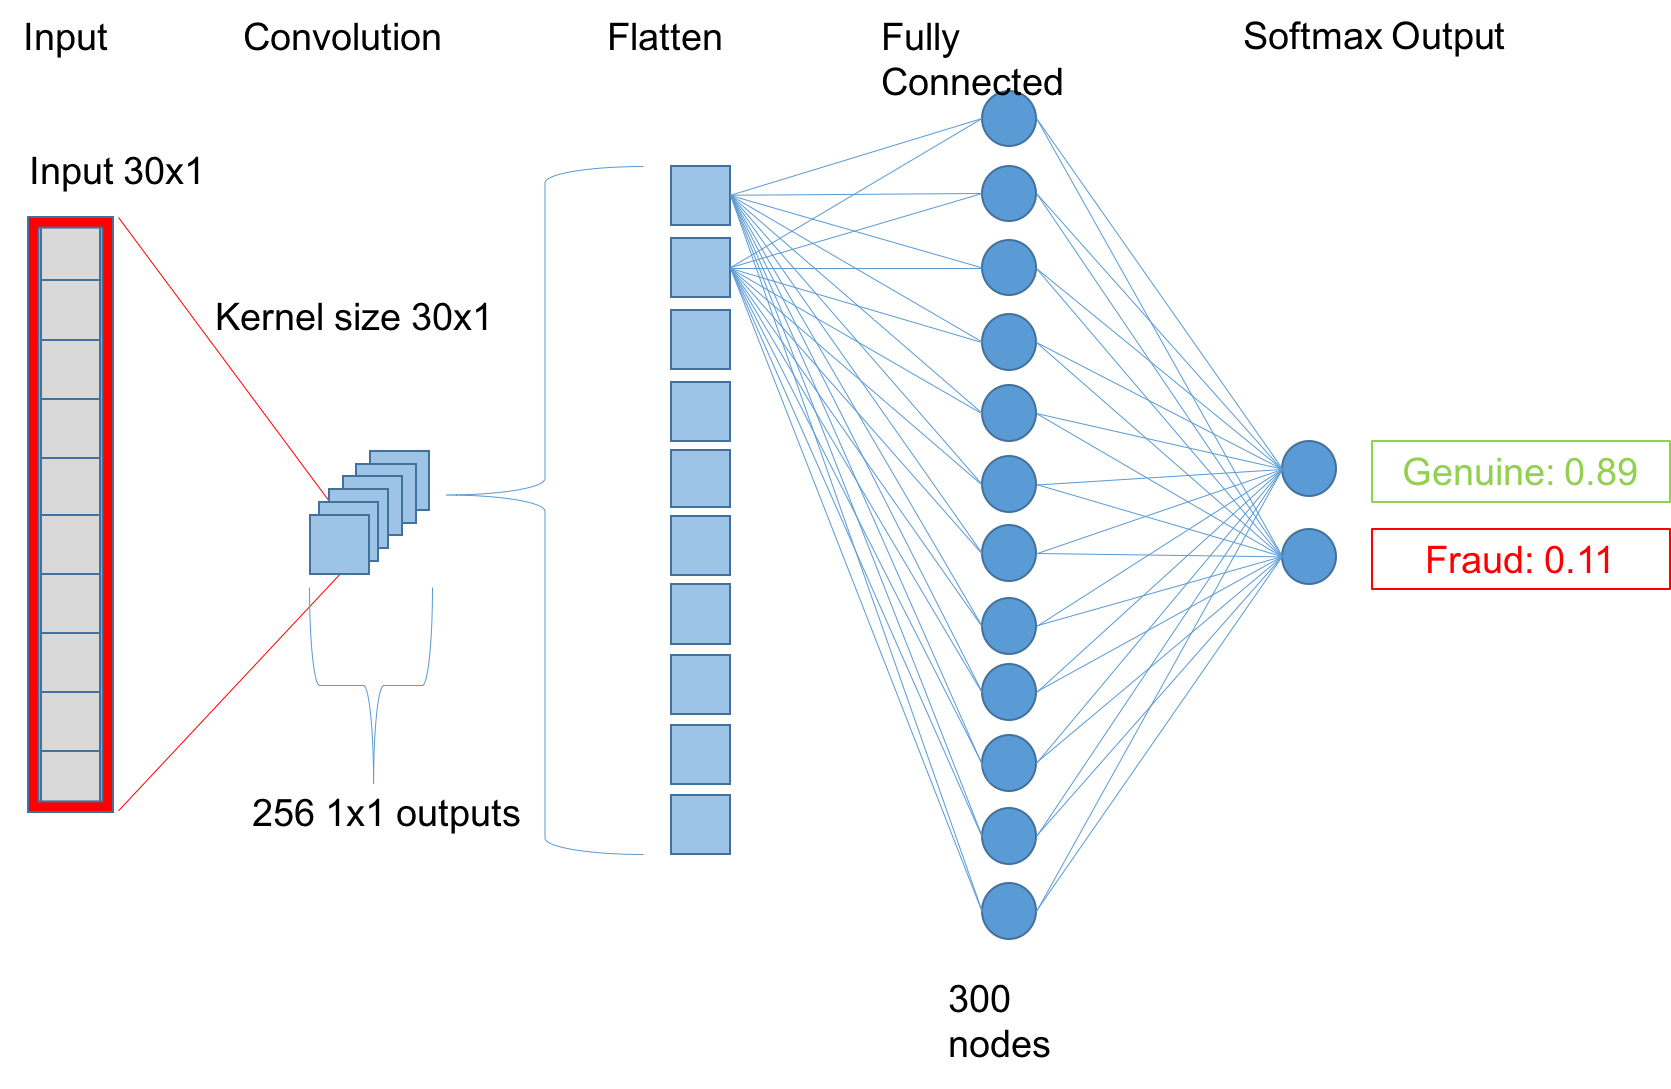
\includegraphics[scale=0.6]{cnnv1}
\caption{Overview of CNN Model 1.}
\label{fig:cnnv1}
\end{figure}

\begin{figure}[H]
\centering
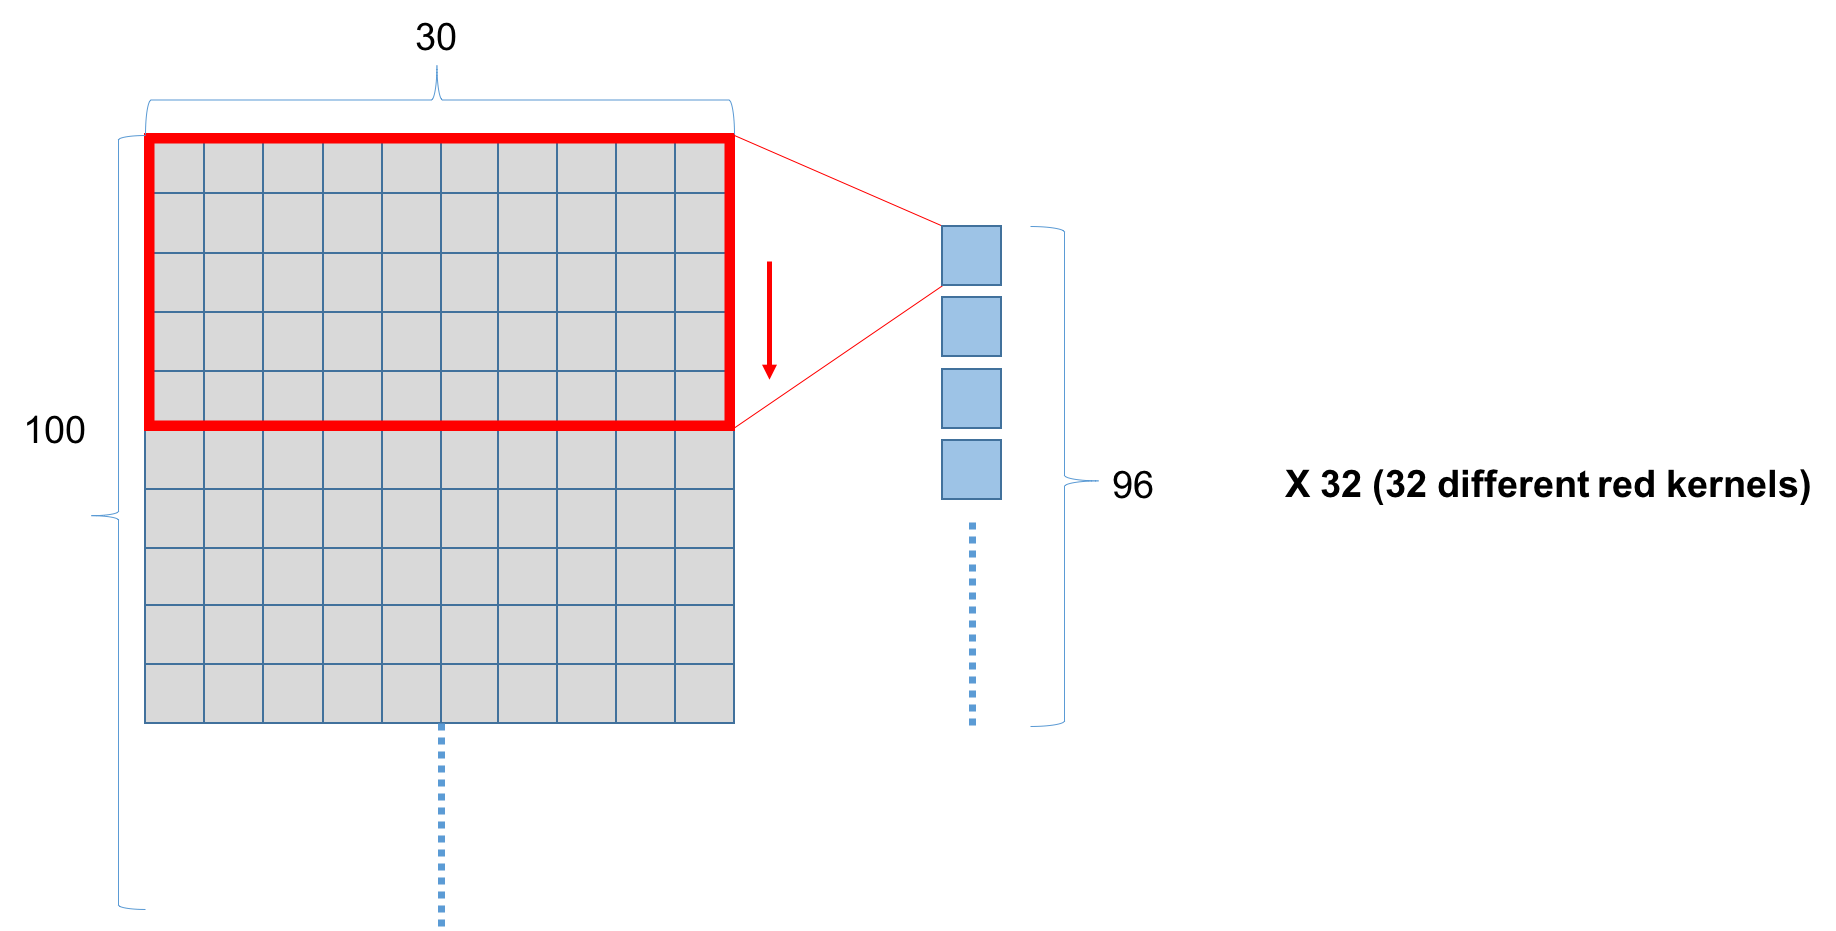
\includegraphics[scale=0.6]{cnnv2-1}
\caption{Overview of CNN Model 2 - Part 1.}
\label{fig:cnnv2-1}
\end{figure}

\subsection{CNN version 2}
\begin{figure}[H]
\centering
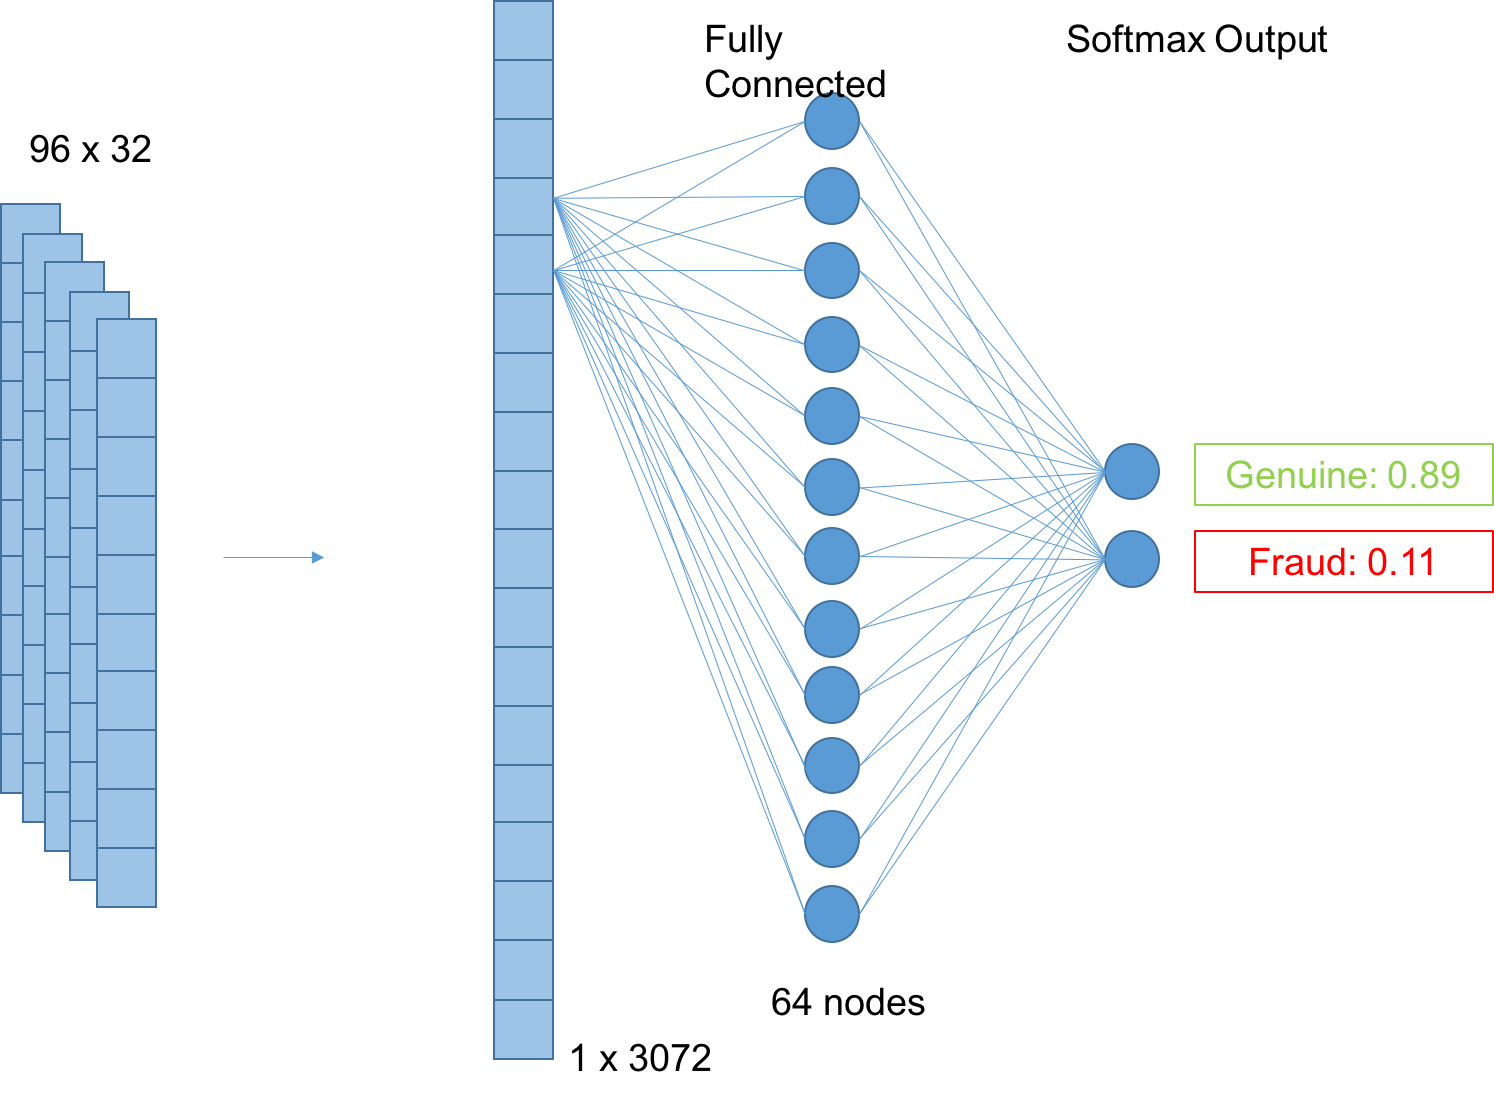
\includegraphics[scale=0.6]{cnnv2-2}
\caption{Overview of CNN Model 2 - Part 2.}
\label{fig:cnnv2-2}
\end{figure}

\section{Generative Adversarial Network Models}

\begin{figure}[H]
\centering
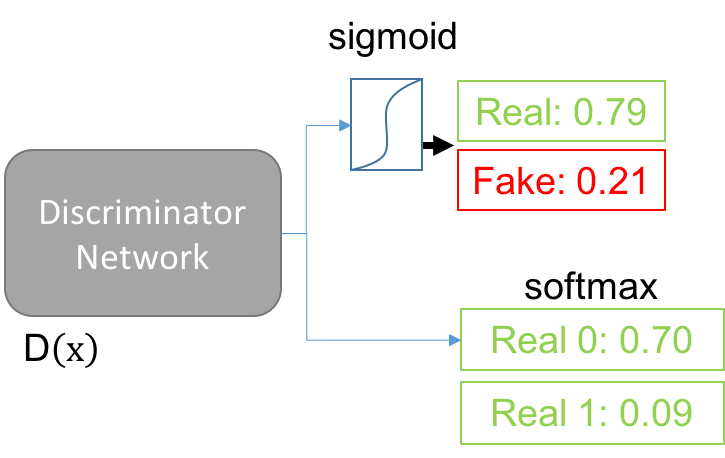
\includegraphics[scale=0.8]{gan-ssl}
\caption{Overview of GAN-SSL discriminator output.}
\label{fig:gan-ssl}
\end{figure}


% Evaluation
\chapter{Evaluation}
\section{Evaluation Methodology}
\subsection{Metrics}
In this project, the metrics that were of interest were not just simply the accuracy, as with many machine learning applications. Accuracy simply measures how many correct classifications are made. This, in the context of credit card fraud, is useless. This is because, even if we classified all fraud as benign, the classifier would still be over 99\% accurate, due to the high imbalance of the fraud/non-fraud classes. In the dataset being used, fraud accounts for only 0.17\% of the total. 

\textbf{Precision and Recall}\\

Therefore we need to look at metrics that tell us more about what we're interested in. Two main measures of interest are \textit{Precision} and \textit{Recall}.

\[
    {Precision} = \frac{T_p}{T_p+F_p} \hspace{5mm} , \hspace{5mm} {Recall} = \frac{T_p}{T_p+F_n} \hspace{1cm}  {T_p} = {True Positive} \hspace{5mm},\hspace{5mm} {F_n} = {False Negative}
\]

Precision is intuitively the ability of the classifier to not misclassify. Recall is intuitively how well to catch fraudulent examples. 

Of course the threshold by which we allow benign transactions to be misclassified as fraud, is a business decision. In the context of a bank, of course the number of fraudulent transactions caught is very important but at the same time we care about precision as this amounts to freezing customers accounts, sending text messages even though they are not subject to fraud, which ultimately costs the bank time and money and potentially customers.

\subsection{Visual Inspections}

\textbf{Precision-Recall Curves and ROC}\\
When classifying, the true positive rate (TPR) and false positive rate (FPR) changes for increasing values of precision and recall. This can be visualised by looking at TPR-FPR curves. This gives an indication of how the trade-off varies for differing values.

Taking the area under this curve is known as AUC, therefore gives an overall statistic for comparing classifiers. 

\textbf{GAN loss function graphs and generated data visualising}\\
With GANs, the way in which we can visualise performance is different to others due to it's specific adversarial nature. Two prominent use cases for GANs is to view the loss function graph for the generator and discriminator networks to see how the two networks fight with each other. In an ideal, theoretical world, we would expect to see the two loss curves converging to some stable value, which indicates the two networks can no longer improve or better themselves. 

Also, seeing as a large part of the GAN architecture is generating data, we can inspect this to see if it looks appropriate. A common example with the MNIST dataset is to see if the generated images look like handwritten digits. In this case, we can inspect the shape and distribution of the generated fraud transactions and view them side-by-side with real fraud transactions to see if any similarities have been picked up by the network.

\section{Results Overview}

% Conclusion
\chapter{Conclusions}

\begin{enumerate}
\item Can you apply DL architectures to this problem? Yes, you can apply them, good/bad? 
\item What can you compare it to, is it useful, how does it
compare
\item What could the recommendation be, would you recommend to use DNN
\end{enumerate}


%%%%%%%%%%%%%%%%%%%%%%%%%%%%%%%%%%%%%%%%%%%%%%%%%%%%%%%%%%%%%%%%%%%%%
% the bibliography
\newpage
\addcontentsline{toc}{chapter}{Bibliography}
\bibliographystyle{ieeetr}
\bibliography{references}

%%%%%%%%%%%%%%%%%%%%%%%%%%%%%%%%%%%%%%%%%%%%%%%%%%%%%%%%%%%%%%%%%%%%%

\end{document}





